\documentclass{article}
\usepackage{listings}

\usepackage{Sweave}
\begin{document}
\Sconcordance{concordance:texProva.tex:texProva.Rnw:%
1 3 1 1 0 10 1 1 2 4 0 1 2 8 1 1 2 8 0 1 2 5 1}



\author{Ottavia}
\title{esempio}

\maketitle

\section{Prova}

\begin{Schunk}
\begin{Sinput}
> x=mean(cars$speed)
\end{Sinput}
\end{Schunk}

15.4

\verb*||

$\sum x_i / n = 15.4$


A nice plot \ref{fig:plot} obtained with ggplot and no effort AT ALL:

\begin{figure}
\caption{Un grafico}
\label{fig:plot}
\centering
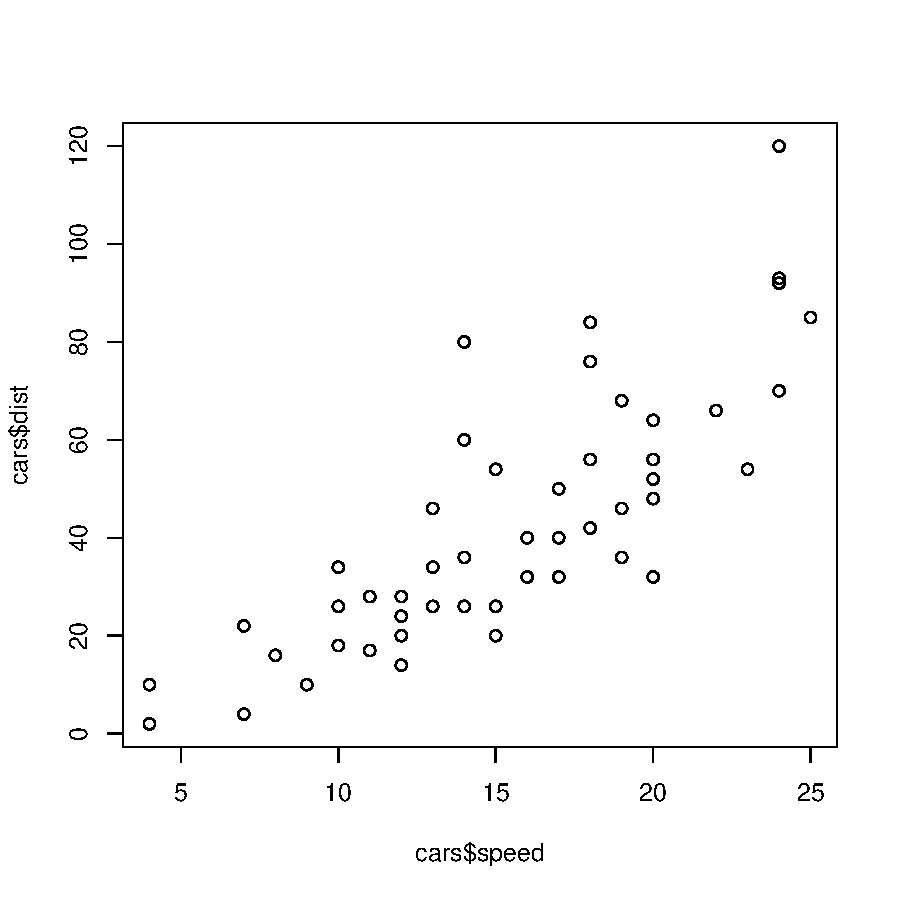
\includegraphics{texProva-002}

\end{figure}

E invece qui abbiamo una bella tabella \ref{tab:table}


\begin{table}[!htbp] \centering 
  \caption{Modello} 
  \label{tab:table} 
\begin{tabular}{@{\extracolsep{5pt}}lc} 
\\[-1.8ex]\hline 
\hline \\[-1.8ex] 
 & \multicolumn{1}{c}{\textit{Dependent variable:}} \\ 
\cline{2-2} 
\\[-1.8ex] & dist \\ 
\hline \\[-1.8ex] 
 speed & 3.932$^{***}$ \\ 
  & (0.416) \\ 
  & \\ 
 Constant & $-$17.579$^{**}$ \\ 
  & (6.758) \\ 
  & \\ 
\hline \\[-1.8ex] 
Observations & 50 \\ 
R$^{2}$ & 0.651 \\ 
Adjusted R$^{2}$ & 0.644 \\ 
Residual Std. Error & 15.380 (df = 48) \\ 
F Statistic & 89.567$^{***}$ (df = 1; 48) \\ 
\hline 
\hline \\[-1.8ex] 
\textit{Note:}  & \multicolumn{1}{r}{$^{*}$p$<$0.1; $^{**}$p$<$0.05; $^{***}$p$<$0.01} \\ 
\end{tabular} 
\end{table} 
E invece qui abbiamo una bella tabella \ref{tab:tabella}


\begin{table}[!htbp] \centering 
  \caption{SUmmary} 
  \label{tab:tabella} 
\begin{tabular}{@{\extracolsep{5pt}}lccccc} 
\\[-1.8ex]\hline 
\hline \\[-1.8ex] 
Statistic & \multicolumn{1}{c}{N} & \multicolumn{1}{c}{Mean} & \multicolumn{1}{c}{St. Dev.} & \multicolumn{1}{c}{Min} & \multicolumn{1}{c}{Max} \\ 
\hline \\[-1.8ex] 
mpg & 32 & 20.091 & 6.027 & 10.400 & 33.900 \\ 
cyl & 32 & 6.188 & 1.786 & 4 & 8 \\ 
disp & 32 & 230.722 & 123.939 & 71.100 & 472.000 \\ 
hp & 32 & 146.688 & 68.563 & 52 & 335 \\ 
drat & 32 & 3.597 & 0.535 & 2.760 & 4.930 \\ 
wt & 32 & 3.217 & 0.978 & 1.513 & 5.424 \\ 
qsec & 32 & 17.849 & 1.787 & 14.500 & 22.900 \\ 
vs & 32 & 0.438 & 0.504 & 0 & 1 \\ 
am & 32 & 0.406 & 0.499 & 0 & 1 \\ 
gear & 32 & 3.688 & 0.738 & 3 & 5 \\ 
carb & 32 & 2.812 & 1.615 & 1 & 8 \\ 
\hline \\[-1.8ex] 
\end{tabular} 
\end{table} 
\begin{verbatim}\label{code:cod1}
\begin{Schunk}
\begin{Sinput}
> y = a + bx + e
\end{Sinput}
\end{Schunk}

\end{verbatim}

\end{document}
